
\chapter{Quantum computers and mapping of quantum circuits}
\label{sec:org9b8733c}

\section{Quantum computing}
\label{sec:org94895bc}

Quantum computers will be able to solve problems that are intractable for classical computers.
Due to the quantum phenomena, quantum computers are able to explore a whole solution space at once.
The most famous example is  Shor's quantum algorithm. It is an integer factorization algorithm able to calculate prime numbers in polynomial time, which is exponentially faster than its classical counterpart, General Number Field Sieve (GNFS). 
In general, quantum computers are a promising technology able to solve problems considered hard in classical computation.
In the next sections we will explain the basics of quantum computation.

\subsection{Essential elements of quantum computation}
\label{sec:orgba4af21}

Quantum bits (or qubits) and quantum gates are the basic ingredients in quantum computation.
As in classical computation with boolean gates and bits, quantum gates operate on the qubits to change their state and return the desired result or calculation.

\begin{enumerate}
\item Qubits
\label{sec:org6bb5ea6}
%% Space

A qubit is the basic unit of information in quantum computing.
A classical bit can be either \texttt{0} or \texttt{1}.
A qubit's state could be either \texttt{0} or \texttt{1} or both at the same time, what is called \textbf{superposition}.
Both, ground or excited states, are represented in the Dirac's bra-ket notation \cite{Nielsen_2009}, \(| 0 \rangle\) and \(| 1 \rangle\) respectively.
A qubit is described as in a probabilistic state \(| \psi \rangle = \alpha_0 | 0 \rangle + \alpha_1 | 1 \rangle\), where \(\alpha_0, \alpha_1 \in \mathbb{C}\) are the so-called probability amplitudes.
\(|\alpha_0|^2\) is the probability of measuring \(| 0 \rangle\) and \(|\alpha_1|^2\) is the probability of measuring \(| 1 \rangle\).
In other words, when a qubit is measured, one can get the measurement result '0' with probability \(|\alpha_0|^2\) and '1' with probability \(|\alpha_1|^2\).
In addition, the qubit's state collapses to either \(| 0 \rangle\) or \(| 1 \rangle\), respectively.
As \(|\alpha_0|^2\) and \(|\alpha_1|^2\)  are probabilities, the sum of them should be \(|\alpha_0|^2 + |\alpha_1|^2 = 1\).
Therefore a qubit state can be represented as a vector (eq. \ref{eq:org1bd4103}).

\begin{equation}
\label{eq:org1bd4103}
|\psi\rangle = \begin{bmatrix}\alpha_0 \\ \alpha_1 \end{bmatrix}
\end{equation}

As soon as the vectors are 2-dimensional, complex and unitary they can also be described in phase notation \cite{Nielsen_2009}.
Like the complex numbers, although requiring two angles in this case.
This notation lead us to an understandable way to visualize the quantum states, the \textbf{Bloch sphere} (fig. \ref{fig:bloch_sphere}).
A sphere of radius one, which z-axis extremes represent the ground and excited states.

\begin{figure}
\centering
\begin{tikzpicture}[line cap=round, line join=round, >=Triangle]
  \clip(-2.19,-2.49) rectangle (2.66,2.58);
  \draw [shift={(0,0)}, lightgray, fill, fill opacity=0.1] (0,0) -- (56.7:0.4) arc (56.7:90.:0.4) -- cycle;
  \draw [shift={(0,0)}, lightgray, fill, fill opacity=0.1] (0,0) -- (-135.7:0.4) arc (-135.7:-33.2:0.4) -- cycle;
  \draw(0,0) circle (2cm);
  \draw [rotate around={0.:(0.,0.)},dash pattern=on 3pt off 3pt] (0,0) ellipse (2cm and 0.9cm);
  \draw (0,0)-- (0.70,1.07);
  \draw [->] (0,0) -- (0,2);
  \draw [->] (0,0) -- (-0.81,-0.79);
  \draw [->] (0,0) -- (2,0);
  \draw [dotted] (0.7,1)-- (0.7,-0.46);
  \draw [dotted] (0,0)-- (0.7,-0.46);
  \draw (-0.08,-0.3) node[anchor=north west] {$\varphi$};
  \draw (0.01,0.9) node[anchor=north west] {$\theta$};
  \draw (-1.01,-0.72) node[anchor=north west] {$\mathbf {\hat{x}}$};
  \draw (2.07,0.3) node[anchor=north west] {$\mathbf {\hat{y}}$};
  \draw (-0.5,2.6) node[anchor=north west] {$\mathbf {\hat{z}=|0\rangle}$};
  \draw (-0.4,-2) node[anchor=north west] {$-\mathbf {\hat{z}=|1\rangle}$};
  \draw (0.4,1.65) node[anchor=north west] {$|\psi\rangle$};
  \scriptsize
  \draw [fill] (0,0) circle (1.5pt);
  \draw [fill] (0.7,1.1) circle (0.5pt);
\end{tikzpicture}
\caption{The Bloch sphere}
\label{fig:bloch_sphere}
\end{figure}

The power of quantum computers comes from the combination of several qubits.
The quantum state of \(n\) qubits can be represented in bra-ket notation, with a \(2^n\) size.
For instance, the state of two and $n$ qubits are represented in the eq. \ref{eq:two_q_state} and \ref{eq:multiple_q_state}, respectively.
Another important quantum property is \textbf{entanglement}, which qubits are correlated with each other.

\begin{equation}
\label{eq:two_q_state}
|\psi\rangle = \alpha_0 |00\rangle + \alpha_1 |01\rangle + \alpha_2 |10\rangle + \alpha_3 |11\rangle
\end{equation}

\begin{equation}
\label{eq:multiple_q_state}
|\psi\rangle = \alpha_0 |0...0\rangle + \alpha_1 |0...1\rangle + ... + \alpha_{n-1} |1...1\rangle
\end{equation}


\item Quantum Operations
\label{sec:org47d83ef}

Quantum operations leverage the power of quantum computers enabling calculations on the qubits.
Quantum operations change the state of the qubit.
We consider three kind of operations in quantum computing: gates, qubits' measurements and qubit initialization processes.
Quantum gates are represented as square matrices of \(2^{n} \times 2^{n}\), where \(n\) is the number of qubits involved in the operation.
This matrices should be unitary respecting the qubit state vector unitary property (\(|\alpha_0|^2 + |\alpha_1|^2 = 1\)).
Single-qubit operations can be represented as state rotations in the Bloch sphere (Fig. \ref{fig:bloch_sphere}).
For instance, an X gate is a rotation of 180° in x-axis of the Bloch sphere and changes the qubit state from \(| 0 \rangle\) to \(| 1 \rangle\), or viceversa.
An example of the matrix representation of a quantum operation and the way to operate with qubits is shown in eq. \ref{eq:inner_prod_ex}.

\begin{equation}
\label{eq:inner_prod_ex}
U |\psi\rangle=\begin{bmatrix}u_{00}&u_{01}\\u_{10}&u_{11}\end{bmatrix} \begin{bmatrix}\alpha_0 \\ \alpha_1 \end{bmatrix} = \begin{bmatrix}\alpha_0 u_{00} + \alpha_1 u_{01} \\ \alpha_0 u_{10} + \alpha_1 u_{11} \end{bmatrix}
\end{equation}


\begin{enumerate}
\item Single-qubit gates
\label{sec:orgdcd22f5}

Single qubit gates operate just on one qubit.
As explained before, single-qubit gates can be represented as \(2^1 \times 2^1\) square matrices that should be unitary.
The symbol and the matrix representation of the most common single-qubit gates can be found in Table \ref{tab:single_q_gates}.

\begin{table}[htbp]
\caption{\label{tab:single_q_gates}
Most common single qubit gates}
\centering
\begin{tabular}{ccccccc}
\hline
Identity & Pauli-X & Pauli-Y & Pauli-Z & Hadamard & S gate & T gate\\
\hline
\Qcircuit @C=1em @R=.7em {
  \lstick{|q\rangle} & \gate{I} & \qw\\
}
 & \Qcircuit @C=1em @R=.7em {
  \lstick{\shortmid q\rangle} & \gate{I} & \qw\\
}
 & \Qcircuit @C=1em @R=.7em {
  & \gate{Y} & \qw\\
}
 & \Qcircuit @C=1em @R=.7em {
  \lstick{|q\rangle} & \gate{Z} & \qw\\
}
 & \Qcircuit @C=1em @R=.7em {
  & \gate{H} & \qw\\
}
 & \Qcircuit @C=1em @R=.7em {
  \lstick{|q\rangle} & \gate{S} & \qw\\
}
 & \Qcircuit @C=1em @R=.7em {
  \lstick{|q\rangle} & \gate{T} & \qw\\
}
\\
\(\begin{bmatrix}1&0\\0&1\end{bmatrix}\) & \(\begin{bmatrix}0&1\\1&0\end{bmatrix}\) & \(\begin{bmatrix}0&-i\\i&0\end{bmatrix}\) & \(\begin{bmatrix}1&0\\0&-1\end{bmatrix}\) & \(\frac{1}{\sqrt{2}}\begin{bmatrix}1&1\\1&-1\end{bmatrix}\) & \(\begin{bmatrix}1&0\\0&i\end{bmatrix}\) & \(\begin{bmatrix}1&0\\0&e^{i \pi / 4}\end{bmatrix}\)\\
\hline
\end{tabular}
\end{table}

The \emph{Identity} gate is the idling operation.
It is equivalent to no applying any operation for a cycle.
The \emph{Pauli-x, -y and -z} gates are 180° rotation over the x-, y- and z-axis, respectively.
The \emph{Hadamard} gate is also a 180° rotation, but over the diagonal axis between the x- and z-axes, \(\frac{({\hat {x}}+{\hat {z}})}{\sqrt {2}}\).
The \emph{S} and \emph{T} gates are also rotations over the z-axis but of 90° and 45° respectively.


\item Two-qubit gates
\label{sec:org2153382}

Two-qubit gates are quantum operations that involve two qubits.
In general, the two-qubit gates execute a single-qubit operation over one of the qubits, depending on the state of the other.
The qubits that goes through the operation is called \textbf{target}, while the other is called the \textbf{control} qubit.
The most common two-qubit gates are represented in Table \ref{tab:two_q_gates}.
The \emph{CNOT} gate is a Controlled-NOT operation or, what is the same, a Pauli-x gate that, depending on the state of the control qubit will be executed or not.
If the control qubit is \(| 1 \rangle\), a Pauli-x will be executed onthe target qubit.
As the CNOT, the \emph{CZ} gate is a Controlled-Z operation that, in this case, performs a Pauli-z gate in the target qubit when the control qubit is \(|1\rangle\).
Finally, the \emph{SWAP} gate exchanges the state of two qubits.
This gate is mostly used for routing purposes as it will be seen in the next sections.

\begin{table}[htbp]
\caption{\label{tab:two_q_gates}
Most common two-qubit gates}
\centering
\begin{tabular}{ccc}
\hline
CNOT & CZ & SWAP\\
\hline
\Qcircuit @C=1em @R=.7em {
  & \targ & \qw\\
  & \ctrl{-1} & \qw\\
}
 & \Qcircuit @C=1em @R=.9em {
  & \ctrl{1} & \qw\\
 & \control \qw & \qw\\
}
 & \Qcircuit @C=1em @R=.7em {
 & \qswap & \qw\\
  & \qswap \qwx[-1] & \qw\\
}
\\
\(\begin{bmatrix}1&0&0&0\\0&1&0&0\\0&0&0&1\\0&0&1&0\end{bmatrix}\) & \(\begin{bmatrix}1&0&0&0\\0&1&0&0\\0&0&1&0\\0&0&0&-1\end{bmatrix}\) & \(\begin{bmatrix}1&0&0&0\\0&0&1&0\\0&1&0&0\\0&0&0&1\end{bmatrix}\)\\
\hline
\end{tabular}
\end{table}

\item Universality
\label{sec:orgaa1dd6c}

A \textbf{universal set of gates} is a set of operations able to generate any other gate by combining them \cite{Nielsen_2009}.
In classical computation, for example, the \texttt{OR} and the \texttt{AND} gates are able to generate any other logic gate.
Also comparable with the boolean gates, quantum operations can be decomposed in other set of quantum operations.
In quantum computation there are several universal set of gates.
The most used one is the \textbf{Clifford+T} set, formed by the Clifford gate set -- phase shifts around the three axes, H and CNOT -- and the T gate.
\end{enumerate}
\end{enumerate}

\subsection{Quantum Circuits}
\label{sec:org836a422}

Quantum algorithms can be described by quantum circuits when the circuit model of computation is adopted.
As mentioned before, they consist of quantum gates and qubits connected in circuit fashion.
As most of the algorithm description models -- no matter if classical or quantum --, quantum circuits are hardware agnostic, which is that they are not specified to any quantum device.
In Fig. \ref{fig:circuit_example} we present an example of a quantum circuit.
This circuit represents the quantum equivalent of a Gray encoder of six bit length.
It is composed by 6 qubits and CNOT gates.

\begin{figure}[H]
    \centering

\resizebox{0.2\textwidth}{!}{
\Qcircuit @C=1em @R=.7em {
\lstick{a} & \targ & \qw & \qw & \qw & \qw & \qw\\
\lstick{b} & \ctrl{-1} & \targ & \qw & \qw & \qw & \qw\\
\lstick{c} & \qw & \ctrl{-1} & \targ & \qw & \qw & \qw\\
\lstick{d} & \qw & \qw & \ctrl{-1} & \targ & \qw & \qw\\
\lstick{e} & \qw & \qw & \qw & \ctrl{-1} & \targ & \qw\\
\lstick{f} & \qw & \qw & \qw & \qw & \ctrl{-1} & \qw
}
}
\caption{Gray encoder quantum circuit.}
\label{fig:circuit_example}
\end{figure}


\subsection{Qubits are faulty}
\label{sec:org9e13eea}
Quantum operations are faulty and qubits are not able to hold the desired state for long times, gradually rotating to another state -- the qubit decoheres.
For instance, in the case of superconducting technologies \cite{O_Brien_2017}, the chips bear with decoherence times of \(\sim 30 \mu s\) for qubit relaxation and \(\sim 60 \mu s\) for qubit dephase.
The error rates of single-qubit gates are less than 0.1\% taking \(> 20 ns\) to be executed, while two-qubit gates error rate is 0.6\% with times of \(40 ns\) and measurement error rates around 1\% with execution times of \(\sim 300 ns\) \cite{O_Brien_2017,Versluis_2017}.
This creates an undesirable environment to compute the most useful algorithms.
Therefore, in order to fight the errors generated by this behaviour, fault-tolerant (FT) and quantum error correction (QEC) mechanisms have been developed during the last years \cite{Nielsen_2009}.

\section{Mapping of quantum circuits}
\label{sec:orgd680d43}
As it was described in the \href{chapter-1.org}{Motivation} section, the mapping step is a critical part of the process to run quantum algorithms.
Quantum algorithms can be described by quantum circuits, that are hardware agnostic and assume any interaction between qubits possible.
They assume the qubits are all-to-all connected.
However, quantum chips have limitations (see \href{chapter-3.org}{Constraints of the Surface-17 chips}).
One of the main constraints is the Nearest Neighbor (NN) constraint.
Instead of connected in an all-to-all fashion, the qubits are arranged in a two-dimensional grid in which connectivity between qubits is limited; each qubit connects at most with four neighbours.
Then, the circuits need a transformation in order to be executed in real quantum device.
This transformation is the so-called mapping process.

The mapping process adapts a quantum circuit representation to the requirements of a real quantum processor.
It brings ideal algorithms down to earth, to the limitations of the quantum chips.
Therefore, the mapping accounts for the realization of quantum algorithms in quantum chips.
In order to do this, the qubit states need to switch places between them -- introducing SWAP gates -- whenever an interaction between two qubits that are not NN is required. 
But, as explained in the previous section (\hyperref[sec:org9e13eea]{Qubits are faulty}), quantum gates are faulty and the longer a circuit is, the more errors appear.
Then, the extra addition of gates or the circuit depth increment due to the mapping task, causes quantum algorithms to accumulate errors and results in more noisy or even useless results.
Therefore, the optimal mapping would be the one that alters the least the original circuit.
In order to address the mapping problem, we split it in three steps: \textbf{scheduling}, \textbf{initial placement} and \textbf{routing}.
These steps can be executed several times, or even continuously, and in any order, depending on the mapping approach.

\subsection{Initial placement}
\label{sec:org839069b}

Throughout this thesis we use the terms \textbf{\emph{virtual} qubits} and \textbf{\emph{physical} qubits} referring to the qubits from the circuit that will be mapped to the real qubits of the quantum chip, respectively.
The initial placement task is responsible to relate the virtual qubits with the physical ones, trying to find the best arrangement in order to minimize non-NN interactions.
As we will see in the example below, an optimal initial placement may help to reduce the number of SWAP gates introduced by the routing step.

\subsection{Routing}
\label{sec:org482e1ff}

When two qubits that need to interact -- i.e. perform a two-qubit gate -- are not NN, they have to be moved or 'routed' to adjacent positions.
The routing process accounts for finding the best path -e.g. shortest path- between two qubits far away in the chip that need to interact.
Qubits (quantum states) can be moved from one position to another by means of SWAP gates.
Therefore, it is a decisive step in order to reduce the number of added gates to the circuit and the circuit depth.

\subsection{Scheduling}
\label{sec:org8b954ea}

A scheduler organizes the circuit operations through the circuit time,
finding whether several operations can be executed in parallel -- at the same time -- or not.
It is possible to schedule in different configurations, for instance As Soon As Possible (\textbf{ASAP}) or As Late As Possible (\textbf{ALAP}), depending on the mapping requirements.

In order to schedule the operations, a dependence graph is built.  A graph that relates qubits and gates sequentially.
Starting from the qubits, it chains all the gates with them.
It is really convenient while mapping, mostly scheduling and finding the parallel operations.
The gates that are in the same graph column can run in parallel.
\subsection{Mapping example}
\label{sec:org9c31051}


In order to illustrate the mapping steps let us consider the following circuit (see Fig. \ref{fig:map_ex_circ}) and the device's chip layout in Fig. \ref{fig:map_ex_chip}, in which circles represent the physical qubits and the edges the connections between them and then possible interactions.  We want to map the Gray code circuit to such as chip layout.
The mapping flow that we will follow starts with a scheduler, then we set the initial placement, route and, finally, we re-schedule in order to make all the gate additions as parallel as possible.
As illustrated in the dependence graph of Fig. \ref{fig:map_ex_depend}, there are no parallel gates.
No better schedule is possible.
Considering the gate times for this device the same ones as the ones described in Tab. \ref{uni_set_gatetime}, the latency of this circuit is 400ns already.


\begin{figure}[H]
\centering
\subfigure[Gray code circuit to map]{
\begin{figure}
\Qcircuit @C=1em @R=.7em {
\lstick{a} & \targ & \qw & \qw & \qw & \qw & \qw\\
\lstick{b} & \ctrl{-1} & \targ & \qw & \qw & \qw & \qw\\
\lstick{c} & \qw & \ctrl{-1} & \targ & \qw & \qw & \qw\\
\lstick{d} & \qw & \qw & \ctrl{-1} & \targ & \qw & \qw\\
\lstick{e} & \qw & \qw & \qw & \ctrl{-1} & \targ & \qw\\
\lstick{f} & \qw & \qw & \qw & \qw & \ctrl{-1} & \qw
}
\end{figure}

\label{fig:map_ex_circ}
}

\subfigure[Dependence graph of the circuit]{
\resizebox{\textwidth}{!}{%
\begin{tikzpicture}

%maximum width= pt
    
    \node [draw, rectangle] (a) at (0,5) {a};
    \node [draw, rectangle] (b) at (0,4) {b};
    \node [draw, rectangle] (c) at (0,3) {c};
    \node [draw, rectangle] (d) at (0,2) {d};
    \node [draw, rectangle] (e) at (0,1) {e};
    \node [draw, rectangle] (f) at (0,0) {f};
    
    \node [draw, ellipse] (cnot1) at (2,4.5) {CNOT a,b};
    \node [draw, ellipse] (cnot2) at (4,3.5) {CNOT b,c};
    \node [draw, ellipse] (cnot3) at (6,2.5) {CNOT c,d};
    \node [draw, ellipse] (cnot4) at (8,1.5) {CNOT d,e};
    \node [draw, ellipse] (cnot5) at (10,0.5) {CNOT e,f};


    \draw (a) -- (cnot1);
    \draw (b) -- (cnot1);
    
    \draw (cnot1) -- (cnot2);
    \draw (c) -- (cnot2);
    
    \draw (cnot2) -- (cnot3);
    \draw (d) -- (cnot3);
    
    \draw (cnot3) -- (cnot4);
    \draw (e) -- (cnot4);
    
    \draw (cnot4) -- (cnot5);
    \draw (f) -- (cnot5);
    
\end{tikzpicture}
}
Latency: 400ns

\label{fig:map_ex_depend}
}


\subfigure[Chip layout where to map the example circuit]{
\resizebox{0.45\textwidth}{!}{%
     \begin{tikzpicture}[x=5mm,y=5mm]
 % \tikzstyle{every node} = [circle, fill=gray!30]
 % \node [green] at (0,0) {[circle, fill=gray!30]};
 \draw node[fill=cyan,circle,minimum size=0.3cm] at (0,0) {};
 % \node [cyan] at (10,0) {\textbullet};
 \draw node[fill=cyan,circle,minimum size=0.3cm] at (10,0) {};
 % \node [green] at (20,0) {\textbullet};
 \draw node[fill=cyan,circle,minimum size=0.3cm] at (20,0) {};
 % \node [red] at (5,5) {\textbullet};
 \draw node[fill=cyan,circle,minimum size=0.3cm] at (5,5) {};
 % \node [red] at (5,-5) {\textbullet};
 \draw node[fill=cyan,circle,minimum size=0.3cm] at (5,-5) {};
 % \node [red] at (15,5) {\textbullet};
 \draw node[fill=cyan,circle,minimum size=0.3cm] at (15,5) {};
 % \node [red] at (15,-5) {\textbullet};
 \draw node[fill=cyan,circle,minimum size=0.3cm] at (15,-5) {};

 \node [purple] at (1,0) {\textbf{2}};
 \node [purple] at (11,0) {\textbf{3}};
 \node [purple] at (21,0) {\textbf{4}};
 \node [purple] at (6,5) {\textbf{0}};
 \node [purple] at (6,-5) {\textbf{5}};
 \node [purple] at (16,5) {\textbf{1}};
 \node [purple] at (16,-5) {\textbf{6}};

 % \draw[{Circle[red]}-Latex] (0,0) -- (2,0);
 \draw[-Latex] (0.1, 0.4)  -- (4.6,4.9);
 %% \draw[-Latex] (0.1, 0.4)  -- (4.6,4.9)   node [midway, above, sloped] {0};
 %% \draw[-Latex] (4.8,4.7)   -- (0.3,0.2)  node [midway, below, sloped] {8};

 \draw[-Latex] (5.4, 4.9)   -- (9.9,0.4);
 %% \draw[-Latex] (5.4, 4.9)   -- (9.9,0.4)  node [midway, above, sloped] {1};
 %% \draw[-Latex] (9.7,0.2) -- (5.2,4.7)   node [midway, below, sloped] {9};

 \draw[-Latex] (10.1,0.4)  -- (14.6,4.9);
 %% \draw[-Latex] (10.1,0.4)  -- (14.6,4.9)  node [midway, above, sloped] {2};
 %% \draw[-Latex] (14.8,4.7)  -- (10.3,0.2) node [midway, below, sloped] {10};

 \draw[-Latex] (15.4, 4.9)  -- (19.9,0.4);
 %% \draw[-Latex] (15.4, 4.9)  -- (19.9,0.4)  node [midway, above, sloped] {3};
 %% \draw[-Latex] (19.7,0.2) -- (15.2,4.7)  node [midway, below, sloped] {11};

 \draw[-Latex] (0.4,-0.1) -- (4.9,-4.6);
 %% \draw[-Latex] (0.4,-0.1) -- (4.9,-4.6)  node [midway, above, sloped] {4};
 %% \draw[-Latex] (4.7,-4.8) -- (0.2,-0.3)  node [midway, below, sloped] {12};

 \draw[-Latex] (5.1, -4.6) -- (9.6,-0.1);
 %% \draw[-Latex] (5.1, -4.6) -- (9.6,-0.1) node [midway, above, sloped] {5};
 %% \draw[-Latex] (9.8, -0.3) -- (5.3, -4.8) node [midway, below, sloped] {13};

 \draw[-Latex] (10.4,-0.1) -- (14.9,-4.6);
 %% \draw[-Latex] (10.4,-0.1) -- (14.9,-4.6) node [midway, above, sloped] {6};
 %% \draw[-Latex] (14.7,-4.8) -- (10.2,-0.3) node [midway, below, sloped] {14};

 \draw[-Latex] (15.1,-4.6) -- (19.6,-0.1);
 %% \draw[-Latex] (15.1,-4.6) -- (19.6,-0.1) node [midway, above, sloped] {7};
 %% \draw[-Latex] (19.8,-0.3)  -- (15.3,-4.8) node [midway, below, sloped] {15};

 \end{tikzpicture}
 }

\label{fig:map_ex_chip}
}


\label{fig:map_ex_def}
\caption{Mapping example draft}
\end{figure}

\begin{enumerate}
\item Initial placement
\label{sec:org4d38c28}


If we place the qubits based on the required interactions -- that is: \(q_1\) next to \(q_2\), \(q_2\) next to \(q_5\) and so on -- we can find in this case a placement in which all qubits can perform the required two-qubit gates.
Then, with an optimal initial placement, we can observe that the circuit could be the same without adding any gate.
No routing would be required.


\begin{figure}[H]
\centering
     \resizebox{0.45\textwidth}{!}{%
     \begin{tikzpicture}[x=5mm,y=5mm]
 % \tikzstyle{every node} = [circle, fill=gray!30]
 % \node [green] at (0,0) {[circle, fill=gray!30]};
 \draw node[fill=cyan,circle,minimum size=0.3cm] at (0,0) {};
 % \node [cyan] at (10,0) {\textbullet};
 \draw node[fill=cyan,circle,minimum size=0.3cm] at (10,0) {};
 % \node [green] at (20,0) {\textbullet};
 \draw node[fill=cyan,circle,minimum size=0.3cm] at (20,0) {};
 % \node [red] at (5,5) {\textbullet};
 \draw node[fill=cyan,circle,minimum size=0.3cm] at (5,5) {};
 % \node [red] at (5,-5) {\textbullet};
 \draw node[fill=cyan,circle,minimum size=0.3cm] at (5,-5) {};
 % \node [red] at (15,5) {\textbullet};
 \draw node[fill=cyan,circle,minimum size=0.3cm] at (15,5) {};
 % \node [red] at (15,-5) {\textbullet};
 \draw node[fill=cyan,circle,minimum size=0.3cm] at (15,-5) {};

 \node [purple] at (2,0) {\textbf{b} $\to$ \textbf{Q2}};
 \node [purple] at (12,0) {\textbf{d} $\to$ \textbf{Q3}};
 \node [purple] at (22,0) {\textbf{f} $\to$ \textbf{Q4}};
 \node [purple] at (7,5) {\textbf{a} $\to$ \textbf{Q0}};
 \node [purple] at (7,-5) {\textbf{c} $\to$ \textbf{Q5}};
 \node [purple] at (17,5) {\textbf{e} $\to$ \textbf{Q1}};
 \node [purple] at (17,-5) {\textbf{6}};

 % \draw[{Circle[red]}-Latex] (0,0) -- (2,0);
 \draw[-Latex] (0.1, 0.4)  -- (4.6,4.9);
 %% \draw[-Latex] (0.1, 0.4)  -- (4.6,4.9)   node [midway, above, sloped] {0};
 %% \draw[-Latex] (4.8,4.7)   -- (0.3,0.2)  node [midway, below, sloped] {8};

 \draw[-Latex] (5.4, 4.9)   -- (9.9,0.4);
%%  \draw[-Latex] (5.4, 4.9)   -- (9.9,0.4)  node [midway, above, sloped] {1};
%%  \draw[-Latex] (9.7,0.2) -- (5.2,4.7)   node [midway, below, sloped] {9};

 \draw[-Latex] (10.1,0.4)  -- (14.6,4.9);
%%  \draw[-Latex] (10.1,0.4)  -- (14.6,4.9)  node [midway, above, sloped] {2};
%%  \draw[-Latex] (14.8,4.7)  -- (10.3,0.2) node [midway, below, sloped] {10};

 \draw[-Latex] (15.4, 4.9)  -- (19.9,0.4);
%%  \draw[-Latex] (15.4, 4.9)  -- (19.9,0.4)  node [midway, above, sloped] {3};
%%  \draw[-Latex] (19.7,0.2) -- (15.2,4.7)  node [midway, below, sloped] {11};

\draw[-Latex] (4.7,-4.8) -- (0.2,-0.3);
%%  \draw[-Latex] (0.4,-0.1) -- (4.9,-4.6)  node [midway, above, sloped] {4};
%%  \draw[-Latex] (4.7,-4.8) -- (0.2,-0.3)  node [midway, below, sloped] {12};

\draw[-Latex] (9.8, -0.3) -- (5.3, -4.8);
%%  \draw[-Latex] (5.1, -4.6) -- (9.6,-0.1) node [midway, above, sloped] {5};
%%  \draw[-Latex] (9.8, -0.3) -- (5.3, -4.8) node [midway, below, sloped] {13};

\draw[-Latex] (14.7,-4.8) -- (10.2,-0.3);
%%  \draw[-Latex] (10.4,-0.1) -- (14.9,-4.6) node [midway, above, sloped] {6};
%%  \draw[-Latex] (14.7,-4.8) -- (10.2,-0.3) node [midway, below, sloped] {14};

\draw[-Latex] (19.8,-0.3)  -- (15.3,-4.8);
%%  \draw[-Latex] (15.1,-4.6) -- (19.6,-0.1) node [midway, above, sloped] {7};
%%  \draw[-Latex] (19.8,-0.3)  -- (15.3,-4.8) node [midway, below, sloped] {15};


 \end{tikzpicture}
 }
\label{fig:map_ex_chip_optim}
}

\label{fig:optimal_init_place}
\caption{Chip layout with the qubits in the optimal initial placement}
\end{figure}


However, if we do a naive initial placement in which, for instance, the virtual qubits ( \(a, b, c\) \ldots{}) are mapped to the physical ones \(Q_0, Q_1, Q_2\) \ldots{} in alphabetical order (see Fig. \ref{fig:map_ex_circ_wrong}).
We will need to start routing them.


\begin{figure}[H]
\centering

\resizebox{0.4\textwidth}{!}{%
     \begin{tikzpicture}[x=5mm,y=5mm]
 % \tikzstyle{every node} = [circle, fill=gray!30]
 % \node [green] at (0,0) {[circle, fill=gray!30]};
 \draw node[fill=cyan,circle,minimum size=0.3cm] at (0,0) {};
 % \node [cyan] at (10,0) {\textbullet};
 \draw node[fill=cyan,circle,minimum size=0.3cm] at (10,0) {};
 % \node [green] at (20,0) {\textbullet};
 \draw node[fill=cyan,circle,minimum size=0.3cm] at (20,0) {};
 % \node [red] at (5,5) {\textbullet};
 \draw node[fill=cyan,circle,minimum size=0.3cm] at (5,5) {};
 % \node [red] at (5,-5) {\textbullet};
 \draw node[fill=cyan,circle,minimum size=0.3cm] at (5,-5) {};
 % \node [red] at (15,5) {\textbullet};
 \draw node[fill=cyan,circle,minimum size=0.3cm] at (15,5) {};
 % \node [red] at (15,-5) {\textbullet};
 \draw node[fill=cyan,circle,minimum size=0.3cm] at (15,-5) {};

 \node [purple] at (2,0) {\textbf{b} $\to$ \textbf{2}};
 \node [purple] at (12,0) {\textbf{d} $\to$ \textbf{3}};
 \node [purple] at (22,0) {\textbf{f} $\to$ \textbf{4}};
 \node [purple] at (7,5) {\textbf{a} $\to$ \textbf{0}};
 \node [purple] at (7,-5) {\textbf{c} $\to$ \textbf{5}};
 \node [purple] at (17,5) {\textbf{e} $\to$ \textbf{1}};
 \node [purple] at (17,-5) {\textbf{6}};

 % \draw[{Circle[red]}-Latex] (0,0) -- (2,0);
 \draw[-Latex] (0.1, 0.4)  -- (4.6,4.9)   node [midway, above, sloped] {0};
 \draw[-Latex] (4.8,4.7)   -- (0.3,0.2)  node [midway, below, sloped] {8};

 \draw[-Latex] (5.4, 4.9)   -- (9.9,0.4)  node [midway, above, sloped] {1};
 \draw[-Latex] (9.7,0.2) -- (5.2,4.7)   node [midway, below, sloped] {9};

 \draw[-Latex] (10.1,0.4)  -- (14.6,4.9)  node [midway, above, sloped] {2};
 \draw[-Latex] (14.8,4.7)  -- (10.3,0.2) node [midway, below, sloped] {10};

 \draw[-Latex] (15.4, 4.9)  -- (19.9,0.4)  node [midway, above, sloped] {3};
 \draw[-Latex] (19.7,0.2) -- (15.2,4.7)  node [midway, below, sloped] {11};

 \draw[-Latex] (0.4,-0.1) -- (4.9,-4.6)  node [midway, above, sloped] {4};
 \draw[-Latex] (4.7,-4.8) -- (0.2,-0.3)  node [midway, below, sloped] {12};

 \draw[-Latex] (5.1, -4.6) -- (9.6,-0.1) node [midway, above, sloped] {5};
 \draw[-Latex] (9.8, -0.3) -- (5.3, -4.8) node [midway, below, sloped] {13};

 \draw[-Latex] (10.4,-0.1) -- (14.9,-4.6) node [midway, above, sloped] {6};
 \draw[-Latex] (14.7,-4.8) -- (10.2,-0.3) node [midway, below, sloped] {14};

 \draw[-Latex] (15.1,-4.6) -- (19.6,-0.1) node [midway, above, sloped] {7};
 \draw[-Latex] (19.8,-0.3)  -- (15.3,-4.8) node [midway, below, sloped] {15};


 \end{tikzpicture}
 }


\label{fig:map_ex_wrong_init}
\caption{Qubit disposition in the chip layout with a naive initial placement}
\end{figure}

\item Routing
\label{sec:orgbffd944}

In order to allow the non-NN qubits to interact, we need to move them to adjacent positions and then we insert SWAPs.
The mapping brings smartly the qubits close to the next operation qubit as well.
For example, it routes \(b\) next to \(a\) but also close to \(c\), avoiding a path increment for the next operation.
The result can be seen in Fig. \ref{fig:map_ex_circ_route}.
After every SWAP, the interchanged virtual qubits appear to follow easily the mapping.
The latency after the routing increases in 1440 ns, \(1440 + 400 = 1840\) ns.


\begin{figure}[H]
\centering
\subfigure[Example circuit routed]{

\resizebox{.5\textwidth}{!}{
    \Qcircuit @C=.5em @R=.7em {
\lstick{a \to Q_0} & \qw & \qw & \targ & \qw & \qw & \qw & \qw & \qw & \qw & \qw & \qw & \qw & \qw & \qw & \qw & \qw & \qw & \qw\\
\lstick{b \to Q_1} & \qswap & \push{d} \qw & \qw & \qw & \qw & \qw & \qw & \qw & \ctrl{2} & \targ & \qw & \qw & \qw & \qw & \qswap & \push{f} \qw & \targ & \qw\\
\lstick{c \to Q_2} & \qw & \qw & \qw & \qswap & \push{f} \qw & \qw & \qw & \qw & \qw & \qw & \qswap & \push{b} \qw & \qw & \qw & \qw & \qw & \qw & \qw\\
\lstick{d \to Q_3} & \qswap \qwx[-2] & \push{b} \qw & \ctrl{-3} & \qw & \qw & \targ & \qswap & \push{c} \qw & \targ & \qw & \qw & \qw & \qswap & \push{f} \qw & \qswap \qwx[-2] & \push{d} \qw & \qw & \qw\\
\lstick{e \to Q_4} & \qw & \qw & \qw & \qw & \qw & \qw & \qw & \qw & \qw & \ctrl{-3} & \qw & \qw & \qw & \qw & \qw & \qw & \ctrl{-3} & \qw\\
\lstick{f \to Q_5} & \qw & \qw & \qw & \qswap \qwx[-3] & \push{c} \qw & \ctrl{-2} & \qswap \qwx[-2] & \push{b} \qw & \qw & \qw & \qswap \qwx[-3] & \push{f} \qw & \qswap \qwx[-2] & \push{c} \qw & \qw & \qw & \qw & \qw
 }
}

\label{fig:map_ex_circ_route}
}

\subfigure[Dependence graph after routing]{

\resizebox{.75\textwidth}{!}{%
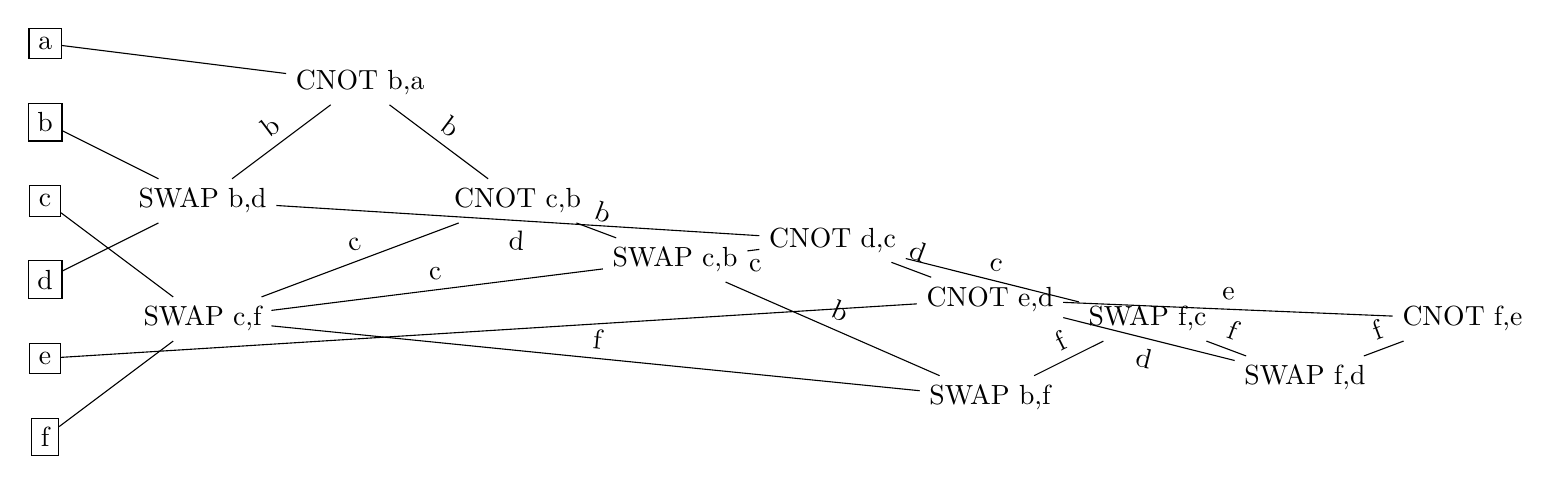
\begin{tikzpicture}
    
    \node [draw, rectangle] (a) at (0,5) {a};
    \node [draw, rectangle] (b) at (0,4) {b};
    \node [draw, rectangle] (c) at (0,3) {c};
    \node [draw, rectangle] (d) at (0,2) {d};
    \node [draw, rectangle] (e) at (0,1) {e};
    \node [draw, rectangle] (f) at (0,0) {f};
    
    \node (swap1) at (2,3) {SWAP b,d};
    \node (swap2) at (2,1.5) {SWAP c,f};
    \node (cnot1) at (4,4.5) {CNOT b,a};
    \node (cnot2) at (6,3) {CNOT c,b};
    \node (swap3) at (8,2.25) {SWAP c,b};
    \node (cnot3) at (10,2.5) {CNOT d,c};
    \node (cnot4) at (12,1.75) {CNOT e,d};
    \node (swap4) at (12,0.5) {SWAP b,f};
    \node (swap5) at (14,1.5) {SWAP f,c};
    \node (swap6) at (16,0.75) {SWAP f,d};
    \node (cnot5) at (18,1.5) {CNOT f,e};
    
    \draw (b) -- (swap1);
    \draw (d) -- (swap1);
    
    \draw (c) -- (swap2);
    \draw (f) -- (swap2);
    
    \draw (a) -- (cnot1);
    \draw (swap1) -- (cnot1) node [midway, above, sloped] {b};
    
    \draw (cnot1) -- (cnot2) node [midway, above, sloped] {b};
    \draw (swap2) -- (cnot2) node [midway, above, sloped] {c};
    
    \draw (cnot2) -- (swap3) node [midway, above, sloped] {b};
    \draw (swap2) -- (swap3) node [midway, above, sloped] {c};
    
    \draw (swap1) -- (cnot3) node [midway, below, sloped] {d};
    \draw (swap3) -- (cnot3) node [midway, below, sloped] {c};
    
    \draw (cnot3) -- (cnot4) node [midway, above, sloped] {d};
    \draw (e) -- (cnot4);
    
    \draw (swap2) -- (swap4) node [midway, above, sloped] {f};
    \draw (swap3) -- (swap4) node [midway, above, sloped] {b};
    
    \draw (cnot3) -- (swap5) node [midway, above, sloped] {c};
    \draw (swap4) -- (swap5) node [midway, above, sloped] {f};
    
    \draw (cnot4) -- (swap6) node [midway, below, sloped] {d};
    \draw (swap5) -- (swap6) node [midway, above, sloped] {f};
    
    \draw (swap6) -- (cnot5) node [midway, above, sloped] {f};
    \draw (cnot4) -- (cnot5) node [midway, above, sloped] {e};
    
\end{tikzpicture}
}

\label{fig:map_ex_depend_resch}
}

\label{fig:map_ex_routing}
\caption{Naive initial placement after routing}
\end{figure}

\item Scheduling
\label{sec:orgeafb033}

As one could notice in the dependence graph (Fig. \ref{fig:map_ex_resch}), there are several operations that can be parallelized.
Therefore, we can apply a scheduling.
In the Fig. \ref{fig:map_ex_resch} the result of an ASAP scheduling is shown, reducing the latency to 1520 ns.
Note that the dashed boxes enclose all the parallel operations in a cycle.



\begin{figure}[H]
\centering

\resizebox{.5\textwidth}{!}{
    \Qcircuit @C=.5em @R=.7em {
 \lstick{a \to Q_0} & \qw & \qw & \qw & \qw & \targ & \qw & \qw & \qw & \qw & \qw & \qw & \qw & \qw & \qw & \qw & \qw & \qw & \qw\\
\lstick{b \to Q_1} & \qswap & \push{d} \qw & \qw & \qw & \qw & \qw & \qw & \qw & \ctrl{2} & \targ & \qw & \qw & \qw & \qw & \qswap & \push{f} \qw & \targ & \qw\\
\lstick{c \to Q_2} & \qw & \qw & \qswap & \push{f} \qw & \qw & \qw & \qw & \qw & \qw & \qw & \qswap & \push{b} \qw & \qw & \qw & \qw & \qw & \qw & \qw\\
\lstick{d \to Q_3} & \qswap \qwx[-2] & \push{b} \qw & \qw & \qw & \ctrl{-3} & \targ & \qswap & \push{c} \qw & \targ & \qw & \qw & \qw & \qswap & \push{f} \qw & \qswap \qwx[-2] & \push{d} \qw & \qw & \qw\\
\lstick{e \to Q_4} & \qw & \qw & \qw & \qw & \qw & \qw & \qw & \qw & \qw & \ctrl{-3} & \qw & \qw & \qw & \qw & \qw & \qw & \ctrl{-3} & \qw\\
\lstick{f \to Q_5} & \qw & \qw & \qswap \qwx[-3] & \push{c} \qw & \qw & \ctrl{-2} & \qswap \qwx[-2] & \push{b} \qw & \qw & \qw & \qswap \qwx[-3] & \push{f} \qw & \qswap \qwx[-2] & \push{c} \qw & \qw & \qw & \qw & \qw \gategroup{1}{2}{6}{5}{.7em}{--} \gategroup{1}{6}{6}{6}{.7em}{--} \gategroup{1}{7}{6}{7}{.7em}{--} \gategroup{1}{8}{6}{9}{.7em}{--} \gategroup{1}{10}{6}{10}{.7em}{--} \gategroup{1}{11}{6}{13}{.7em}{--} \gategroup{1}{14}{6}{15}{.7em}{--} \gategroup{1}{16}{6}{17}{.7em}{--} \gategroup{1}{18}{6}{18}{.7em}{--}
 }
}

\caption{Naive initial placement routed and re-scheduled}
\label{fig:map_ex_resch}
\end{figure}


We summarize the results of using a naive and an optimal initial placement in terms of number of gates and latency in Tab. \ref{tab:optima_vs_naive}.


\begin{table}[htbp]
\caption{\label{tab:optima_vs_naive}
Difference between the naive initial placement and the optimal one in terms of number of operations and latency}
\centering
\begin{tabular}{ccc}
\hline
 & Optimal approach & Naive apprach\\
\hline
\# operations & 5 & 11\\
latency & 400 ns & 1520 ns\\
\hline
\end{tabular}
\end{table}
\end{enumerate}

\section{State of the art on the mapping of quantum circuits}
\label{sec:orgcc4f1c8}
Quantum algorithms are meant to leverage the promising power of quantum computers \cite{coles18:quant_algor_implem_begin}.
Commonly described as quantum circuits, quantum algorithms are hardware agnostic.
However, as we have seen they need to be adapted -- mapped -- to the quantum device limitations.
The main constraints in all of them is the limited connectivity between qubits.
There is a vast amount of literature on the algorithms -- high abstraction level --, neglecting hardware constraints.
From ion traps [? paper on ion traps] to superconducting qubits \cite{Barends_2014,Versluis_2017}, through quantum dots \cite{Hill_2015,Li_2018}, each layout has its own requirements and constraints.
Although all of them are arranged in a 2D -- planar -- structure, ion traps technologies are capable to connect the qubits in all-to-all networks while superconducting technologies connections form a grid shaped network where each qubit is connected to a maximum of four neighbors.
This grid structure establishes one of the main connectivity limitation in today's quantum chips, the NN constraint.
Also industry's superconducting chip layouts from IBM \cite{IBM_QX}, Google \cite{boixo16:charac_quant_suprem_near_term_devic} and Rigetti \cite{Sete_2016} follow this structural limitations.
As for the high abstraction level of the quantum algorithm, a link between the algorithms and the devices is required \cite{Fu_2016}.
As in classical computation, the algorithms should go through a transformation process in order to adapt them to the hosting device.
Certainly, the mapping procedure is an important element of this process.

There is a considerable amount of literature on the mapping task.
Initial works on this field \cite{Metodi_2006,Whitney_2007,Bahreini_2015} focused primarily on the definition of what they characterized as a \emph{scheduler} able to parallelize operations and add the required gates to route qubits.
They consider general connectivity constraints as the NN one, common for most of the devices -- although the works were examining ion-traps as hardware implementations.
The proposed techniques by these works examine a dependency graph looking for the best way to organize qubits and operations.
The majority of the methods use latency as the metric to minimize, however some of them \cite{Farghadan_2017} would minimize in number of SWAP operations.
As it will be explained in the next section, to minimize in latency stands for time optimization while minimize in number of SWAP operations means to find the path that introduces the minimal number of SWAP operations.
Following a similar reasoning as the first approaches, more complex solutions \cite{booth18:compar_integ_const_progr_tempor} have been published using Constraint Programming together with temporal planning, optimizing in latency as well.
Also, several publications \cite{Lye_2015,Wille_2016} outline only the routing sub-task using the number of SWAPS as the metric to minimize.

A recent review of the literature on the mapping topic focused on mapping quantum algorithms on a specific quantum device.
In all the cases, taking into account the specific chip connectivity constrain.
IBM's chip have been gaining much attention due to the open online tools that make the chips accessible to everybody.
Various approaches to mapping algorithms for the IBM family of chips have been proposed \cite{zulehner17:effic_method_mappin_quant_circuit,Siraichi_2018,mckay18:qiskit_backen_specif_openq_openp_exper,Dueck_2018}.
Zulehner et. al \cite{zulehner17:effic_method_mappin_quant_circuit} developed a routing algorithm that optimizes in the number of SWAPs building a graph -- similarly to previous works --  and searching the best route in the chip layout with the A* algorithm.
Siraichi et. al \cite{Siraichi_2018} work defines a weighted dependence graph where the mapping algorithm is able to find a solution for all the mapping steps, initial placement, scheduling and routing.
Also, apart from the works related to the IBM devices, Rigetti's devices have been approached \cite{Venturelli_2018}.

Many attempts have been made \cite{Dousti_2014,Heckey_2015,hwang18:hierar_system_mappin_large_scale,murphy18:contr,Lao_2018} with the purpose of develop a FT mapping able to work at the logical -- qubit -- level.
However, due to the high complexity of the QEC techniques, quantum chips with large amounts of qubits are still theory.
Current and near-future quantum processors are what Preskill \cite{Preskill_2018} calls Noisy Intermediate-Scale Quantum (NISQ) devices; chips with an amount of 50-100 qubits and without QEC or much simpler encodings.
Several studies, for instance \cite{tannu18:case_variab_aware_polic_nisq,paler18:nisq,paler18:influen_initial_qubit_placem_durin}, have been conducted on the mapping algorithms required for NISQ devices.
Also, the works on device specific solutions \cite{zulehner17:effic_method_mappin_quant_circuit,Siraichi_2018,mckay18:qiskit_backen_specif_openq_openp_exper,Dueck_2018,Venturelli_2018} described before, could be considered part of the NISQ works collection.

Besides latency and the number of operations that serve to analyze the quality of a mapping algorithm, few studies have been published on quantum metrics.
In this thesis, we will propose another metrics to evaluate the mapping process.
Fidelity has been addressed in order to characterize the error of a quantum circuit based on the qubits state \cite{Jozsa_1994,Nielsen_2009}.
And, recently, Quantum Volume has been defined to assert the capability of a quantum computer \cite{Moll_2018}.
In the next section and in the \href{chapter-3.org}{New metrics} section we offer an overview of the important metrics in this work.

\section{Mapping metrics}
\label{sec:orgc729465}
As outlined in the state of the art, the literature considers mainly two metrics to optimize in their mapping algorithms and as an output to evaluate how good the mapping is.
These are the added \textbf{latency} and the \textbf{number} of introduced \textbf{operations} after the mapping procedure.
The routing step from the mapping process introduces SWAP gates in the quantum circuit in order to move the qubits around.
And latency is the time required to run a quantum circuit in a given quantum device.
It depends on the chip cycle time and the \textbf{depth} of the circuit, \(Latency = depth \times t_{cycle}\).
Depth is the number of cycles the algorithm encloses.
Actually, most of the studies \cite{Metodi_2006,Whitney_2007,Bahreini_2015} assert the latency in terms of circuit depth, avoiding the cycle time specification of any device.
E.g. in Fig. \ref{fig:latency_swaps_ex}, one can see how after some mapping process some SWAP operations have been added as well as the depth of the circuit or latency grows.
From five cycles depth in the original circuit to nine cycles.


\subsection{Number of SWAPs}
\label{sec:orgaf1dc29}

As explained before in the \hyperref[sec:orgd680d43]{Mapping of quantum circuits} section, to route means to introduce SWAP operations -- or a decomposition of them.
Whenever a two-qubit gate requests two qubits that are far apart, a path in the gridlike chip layout should be given.
Each step on this grid would mean a SWAP operation between the vertex qubits of that step.
We already know that quantum gates are error prone and that one of the main problems that the mapping task is dealing with is to use the least amount of gates as possible.
Although the general mapping problem is to avoid the introduction of error to the original algorithm, that is caused by more sources apart from the number of gates.
Nonetheless, the quantum gates is one of the main error sources altogether with the decoherence time.
That is the reason why the number of SWAPs is commonly used to assert the quality of a mapper, but it is not enough.

The number of SWAPs does not give any information about how long the circuit is, or how much it will be affected by decoherence.
The higher number of SWAPs does not mean the longer the circuit necessarily.
The SWAPs can be in parallel, for instance.
It could be the case of a short circuit with a long number operation in parallel.

\subsection{Latency}
\label{sec:org651820a}

Latency is the time required to run a quantum circuit in a given quantum device.
The introduction of gates due to the mapping makes the target circuit longer.
Or what is the same, the introduction of SWAPs -- or their decomposition -- adds several cycles to the depth of the circuit.
Therefore, the latency of the circuit increases.
For instance, in the \hyperref[sec:org9c31051]{Mapping example}, we can see how the latency grows after the circuit is routed to 1840 ns and then it is reduced to 1520 ns after re-scheduling.



One of the main source of errors is the decoherence, that is the quantum phenomena that makes the qubits loose their state along time.
The longer a quantum device is running an algorithm, the more errors would appear.
Or what is the same, the longer the circuit, the more erroneous will be the result.
The task of the scheduler -- one of the three mapping steps -- is to look for gates that can be run in parallel.
Considering that time is one of the main error sources and that the scheduler task is to make operations simultaneously, one can understand why latency is used in order to assert the capacity of mapping algorithm.
Nonetheless, as the number of SWAPs this metric is not giving enough information for that.

The latency of a circuit gives an intuition of how long it is but, unlike the number of operations, it gives no information about the number of operations it has.
And, therefore, it gives no intuition about how the gate errors are affecting the algorithm final result.

\subsection{Criticism}
\label{sec:org4a19018}

The ideal mapping would be the one affecting the least as possible the original circuit or, what is the same, introducing the least amount of errors.
Clearly, both, latency and number of SWAPs, are direct effects of the mapping procedure that have an impact in the error increase as well.
To optimize in any of them stands on correct -- but not sufficient -- reasoning.
Latency optimization assumes that the most important error source comes from the qubit lifetime.
And, indeed, time is a main issue in quantum computing.
Decoherence time is not only a maximum qubit lifetime, it is harder and harder to hold a quantum state for use times closer to the decoherence time.
On the other hand, to optimize in number of SWAPs stands on the intuition that the gate error is the prominent error in a quantum device.
Although intuitively one can think that the more operations are in a circuit, the longer it will be; as seen in the \href{chapter-1.org}{Problem Statement} section, the higher the number of operations does not necessarily mean the longer circuit depth.
Several operations can be run in parallel in the same cycle -- at the same time.
Actually, to minimize in latency is to maximize in parallelism.
Therefore, even though related, to optimize in one or the other holds different baselines.

Nonetheless, these metrics are not enough to assert how good the mapping process is.
These metrics do not tell you how the algorithm is affected by them.
In other words, my algorithm will still produce good results after the mapping.
They are related with the error rate increase but the relationship is not totally clear.
For instance, it could be the case that concatenation of errors introduced by contiguous gates would end up in a correction of the first error.
Or, that the busier the qubit is, the less affected by decoherence would be.
Then, one question arises.
What would be the best metric?
Definitely, the optimal solution would be to optimize directly in terms of the error rate.
But, in order to do that, a precise prediction of the error should be done and this is a hard computational task in quantum computing.

In this thesis we will analyze how the mapping quality is affected by the different metrics.
Moreover, we will try to find out the best circuit parameter to work as a quality metric of the mapping algorithms.
To perform the analysis we will map several small quantum algorithms on the superconducting quantum chip develop at Qutech by DiCarlo's group 
\cite{Versluis_2017}.
In the next chapter, we will explain the constraints of this chip and the mapping model we will use.
